\documentclass{article}
\usepackage{amsmath,amssymb,amsthm,mdframed,kotex,paralist}
\usepackage{tabto}
%\TabPositions{0.5\textwidth}
\TabPositions{0.33\textwidth,0.66\textwidth}
\newcommand\bp[1]{\begin{mdframed}[frametitle={#1},skipabove=10pt,skipbelow=20pt,innertopmargin=5pt,innerbottommargin=40pt]}
\newcommand\ep{\end{mdframed}\par}
\newcommand\ov[1]{\ensuremath{\overline{#1}}}

\begin{document}
\title{심화문제들(중학교 1학년--중학교 1학년)}
\author{}
\date{\today}
\maketitle

\bp{01}
일차방정식 \(\frac12x+b=0\)의 해가 \(4\)일 때, \(b\)의 값을 구하시오.
\vspace{0.05\textheight}
\ep

\bp{02}
\(|x|+|x-1|=x+7\)의 모든 해의 합을 구하시오.
\vspace{0.3\textheight}
\ep
%
%\bp{03}
%\(1+\frac1{1+\frac1{1+\frac1{1+\frac1{1+\frac1{\cdots}}}}}\)의 값을 구하시오.
%\ep

\bp{03}
\(36\)의 모든 약수의 합을 구하시오.
\vspace{0.1\textheight}
\ep

\bp{04}
\(\frac{220}{2n+1}\)이 정수가 되도록 하는 정수 n의 값은 몇 개 인지 구하시오.
\vspace{0.1\textheight}
\ep

\bp{05}
정수 \(a\), \(b\), \(c\)에 대하여 \(a+\frac3b=1\), \(b+\frac1c=3\)일 때, \(|abc|\)의 값을 구하시오.
\vspace{0.2\textheight}
\ep

\bp{06}
부등식 \(-x+5<3\)을 푸시오.
\ep

\bp{07}
부등식 \(2|x-1|+3|x+1|<6\)을 푸시오.
\vspace{0.3\textheight}
\ep
%
%\bp{08}
%\((a+b)x+(2a-3b)<0\)의 모든 해가 \(3x+1>0\)의 해와 같을 때, \((a-3b)x+(b-2a)>0\)의 해를 구하시오.
%\ep
\newpage
\bp{09}
일차함수 \(y=ax+1-a\)가 4사분면을 지나지 않기 위한 \(a\)의 범위를 구하시오.
\vspace{0.3\textheight}
\ep

\bp{10}
함수 \(y=f(x)\)에 대하여 \(f(ab)=f(a)+f(b)\)가 성립하고 \(f(2)=\frac12\)일 때 \(2f(1)+f(\frac12)\)의 값을 구하시오.
\vspace{0.2\textheight}
\ep

\bp{11}
두 개의 주사위를 던질 때 나온 눈의 합이 5 이하이기 위한 확률을 구하시오.
\vspace{0.2\textheight}
\ep

\bp{12}
한 변의 길이가 2인 정사각형 안에서 무심코 한 점을 찍을 때, 이 점으로부터 사각형의 네 꼭지점까지의 거리가 모두 1보다 클 확률을 구하시오.
\vspace{0.35\textheight}
\ep

\bp{13}
다음 원뿔의 겉넓이를 구하시오.
\par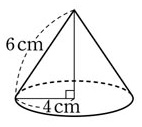
\includegraphics[width=0.3\textwidth]{cone}
\ep

\bp{14}
다음 그림의 평행사변형의 넓이가 \(S\)일 때, 어두운 부분의 넓이를 \(S\)로 나타내어라.
\par\center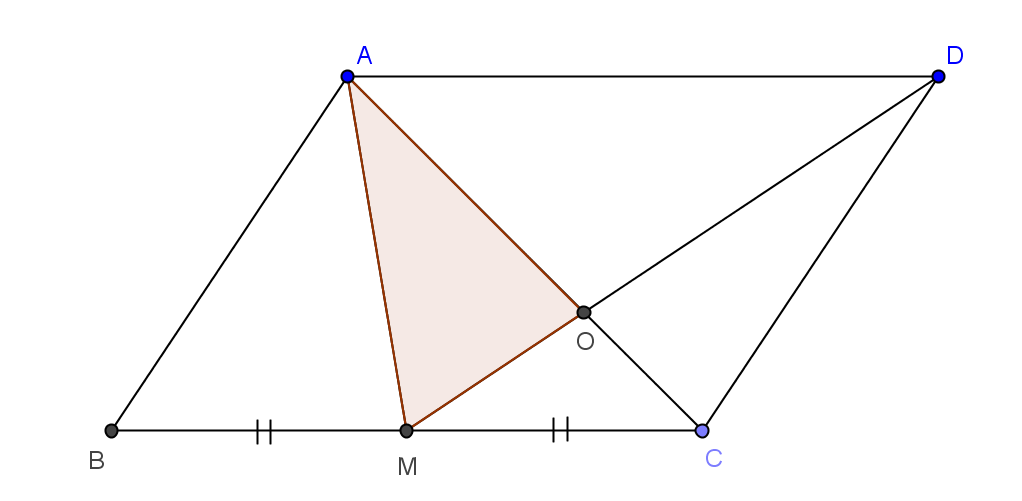
\includegraphics[width=0.8\textwidth]{par}
\ep



\end{document}